%
\subsection{\maxSat\ Example: Details}%
\pdfbookmark[2]{\maxSat\ Example: Details}{maxSatExampleDetails}%
%
%%
\gdef\maxSatClauses{\textcolor{red}{\ensuremath{k}}}%
\gdef\maxSatVariables{\textcolor{green}{\ensuremath{n}}}%
\gdef\maxSatVariable{\ensuremath{x}}%
\gdef\maxSatVariablei#1{\ensuremath{\maxSatVariable_{#1}}}%
\gdef\maxSatFormula{\ensuremath{B}}%
%%
\begin{frame}[label=maxSatDemoStart]%
\frametitle{\maxSat: Output and Analysis}%
\centering{\LARGE{\textbf{\alert{\maxSat: Output and Analysis}}}}%
\bigskip\begin{itemize}%
\item Here we discuss the details of the \maxSat\ example%
\item The following slides can replace the demo, if for some reason running the demo is not possible or did not work out\dots%
\item The evaluation aspects are part of this example.%
\end{itemize}%
\bigskip%
\centering\scalebox{1.8}{\hyperlink{maxSatInteractiveDemoStart}{\beamergotobutton{go back to interactive demo slides}}}%
\end{frame}%
%%
%
\begin{frame}[t]%
\frametitle{ECDF}%
\begin{itemize}%
\item We can plot the Empirical (Cumulative) Distribution Function (ECDF)\scitep{HAFR2012RPBBOBES,HS1998ELVAPAR,TH2004UAIAEEFSAFSAMS,WCTLTCMY2014BOAAOSFFTTSP} for us, which provides the fraction of runs that have found the solution for their respective problem at a given point in time.%  
\end{itemize}%
%
\locateWithCaption{2-6}{%
\strut\vbox to 0.475\paperheight{\vfil%
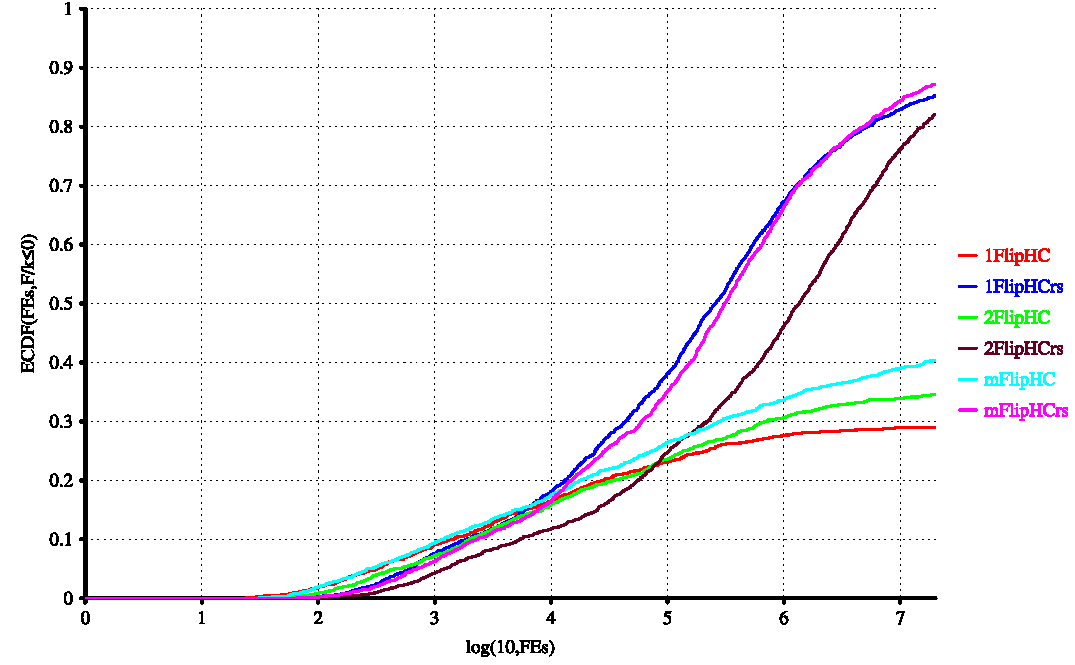
\includegraphics[scale=0.425]{graphics/maxsat_example/ECDF_log_10_FEs_F_k_0/IEEEtran_ECDF_log_10_FEs_F_k_0}%
\strut\hfill\strut%
}%
}{%
The ECDF in over all 100 benchmark instances for time measure \measureFEs\ (log-scaled\only<6->{\alert{, optimized for \texttt{IEEEtran} and two figures per row}}).%
}{0.0375}{0.34}{0.925}%%
%
\locateWithCaption{7}{%
\strut\vbox to 0.475\paperheight{\vfil%
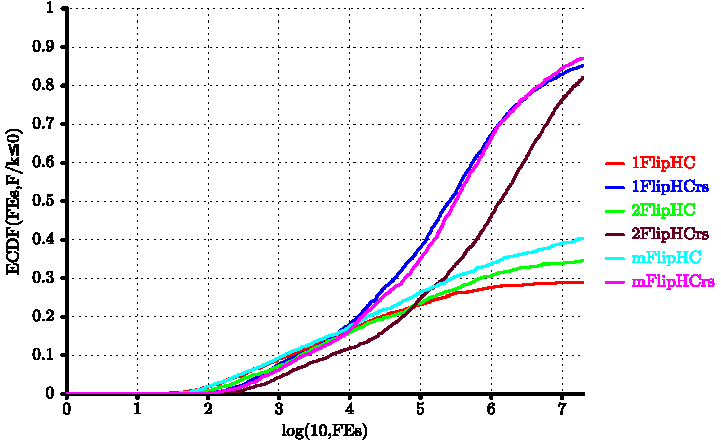
\includegraphics[scale=0.425]{graphics/maxsat_example/ECDF_log_10_FEs_F_k_0/LNCS_ECDF_log_10_FEs_F_k_0}%
\strut\hfill\strut}%
}{%
The ECDF in over all 100 benchmark instances (log-scaled, \alert{optimized for \texttt{LNCS} and two figures per row}).%
}{0.0375}{0.34}{0.925}%
%
\locateWithCaption{8}{%
\strut\vbox to 0.475\paperheight{\vfil%
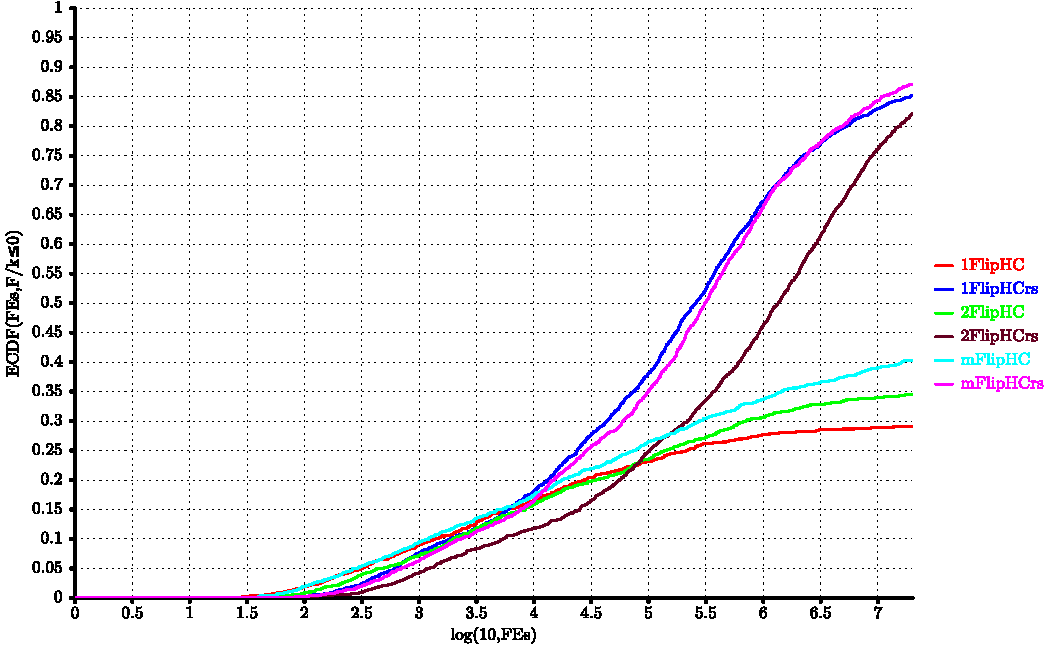
\includegraphics[scale=0.425]{graphics/maxsat_example/ECDF_log_10_FEs_F_k_0/SigAlternate_ECDF_log_10_FEs_F_k_0}%
\strut\hfill\strut}%
}{%
The ECDF in over all 100 benchmark instances (log-scaled, \alert{optimized for \texttt{sig-alternate} and two figures per row}).%
}{0.0375}{0.34}{0.925}%
%
\locateWithCaption{9}{%
\strut\vbox to 0.475\paperheight{\vfil%
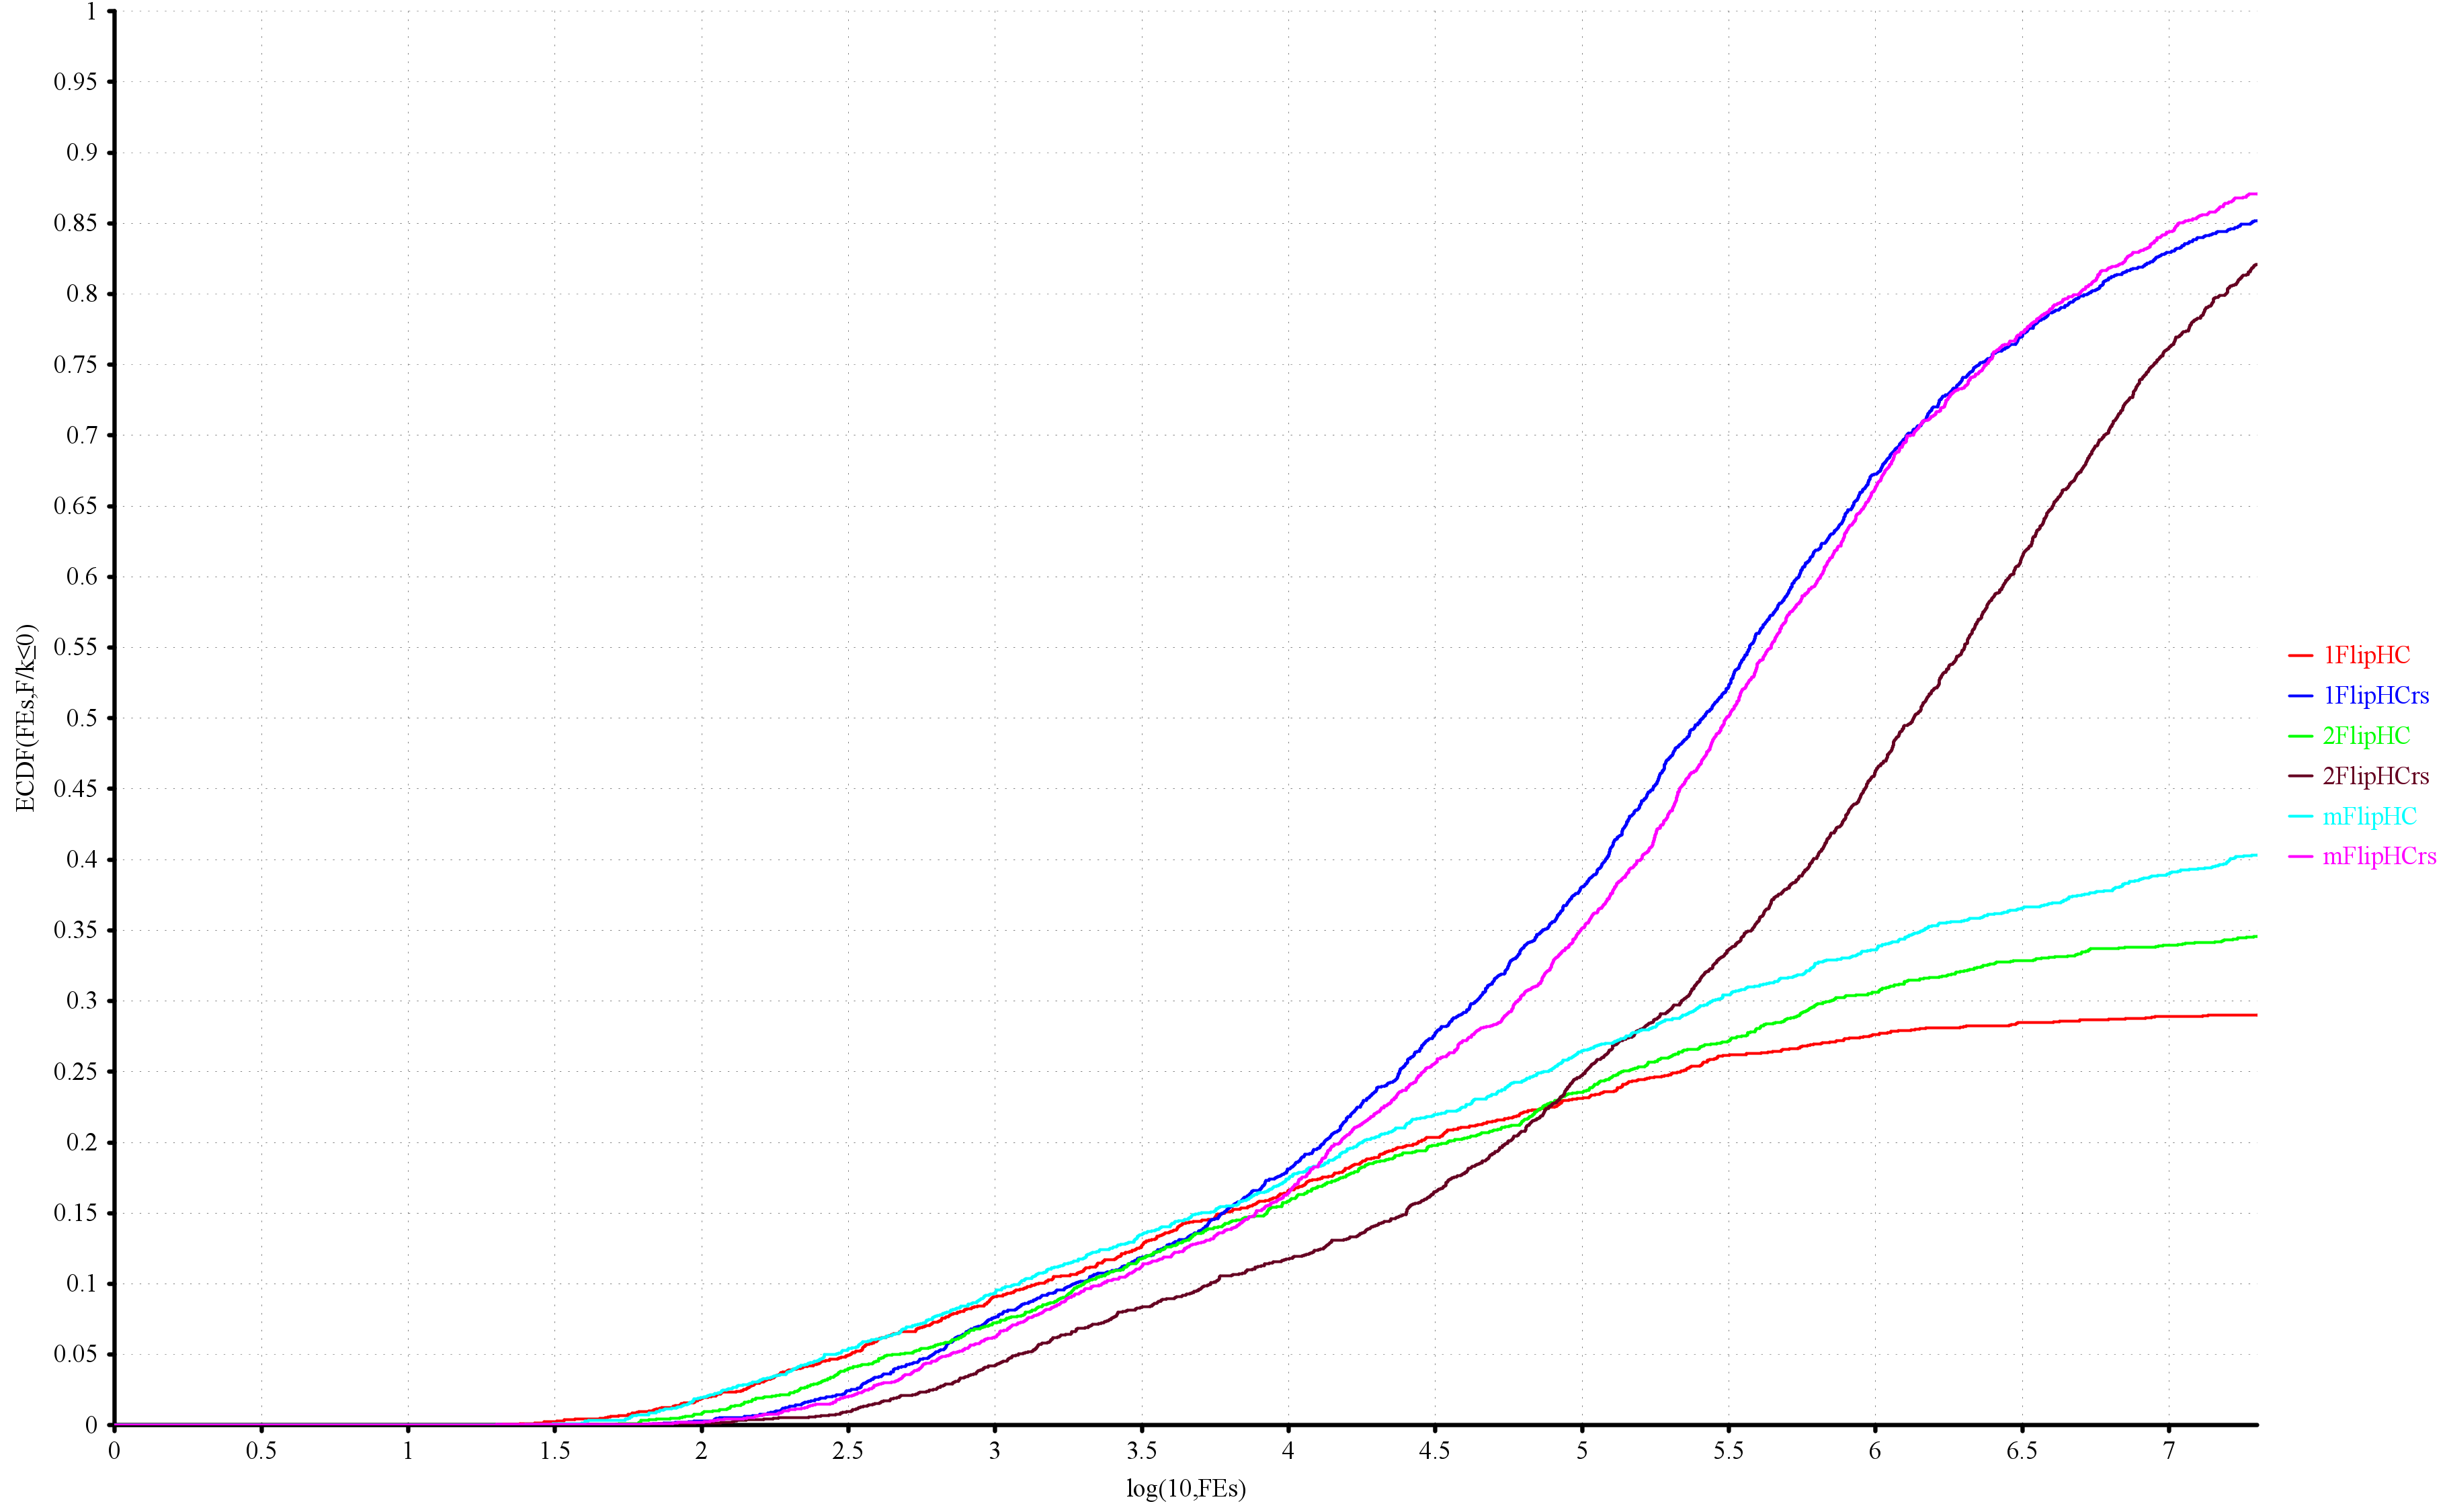
\includegraphics[width=0.6\paperwidth]{graphics/maxsat_example/ECDF_log_10_FEs_F_k_0/XHTML_ECDF_log_10_FEs_F_k_0}%
\strut\hfill\strut}%
}{%
The ECDF in over all 100 benchmark instances (log-scaled, \alert{optimized for \texttt{XHTML} and two figures per row}).%
}{0.0375}{0.34}{0.925}%
%
\locate{3-}{\parbox{0.35\paperwidth}{\small%
\begin{itemize}%
\item the methods with restarts solve more problems (up to 90\%!)%
\item<4-> plain $m$-flips are better than 2-flips are better than 1-flips%
\item<5-> oddly, for restart HCers, there is a tie between the $m$- and 1-flip versions 
\end{itemize}%
}}{0.625}{0.3}%
%
\end{frame}%
%
\begin{frame}%
\frametitle{ECDF for Different Values of \scalebox{1.3}{\ensuremath{\mathbf{\maxSatVariables}}}}%
%
\locate{1-}{%
\parbox{0.234\paperwidth}{\raggedright\small{%
\only<-1>{We now look at the ECDF for different values of \maxSatVariables\ and a goal of 1\% unsatisfied clauses over \measureRuntime\ (log-scaled).}%
\only<2>{For $\maxSatVariables=20$, the methods with restarts are better.}%
\only<3>{But for $\maxSatVariables\geq 50$, those without reach the goal faster.}%
\only<4>{It seems that 1\% unsatisfied clauses can be reached with 1-flips and without restarts.}%
\only<5>{The 2-flip operator again performs worst.}%
\only<6>{It looks as if it gets easier to attain a 1\% error margin if \maxSatVariables\ increases (all ECDFs reach 1).}%
\only<7-8>{For small problems, 1-flip is slightly faster than $m$-flip.}%
\only<9>{For larger problems, $m$-flip becomes slightly faster.}%
\only<10>{All in all, similar behavior over all scales (reaching 1\% error seems to be easy).}%
\only<11->{Only required runtime increases by up to 100 times.}%
}}}{0.013}{0.187}%
%
\locate{1-}{%
\parbox{0.234375\paperwidth}{\centering%
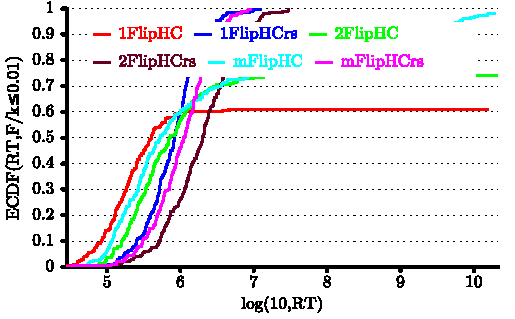
\includegraphics[width=0.234375\paperwidth]{graphics/maxsat_example/ECDF_log_10_RT_F_k_0_01_distinct_n/SigAlternate_ECDF_log_10_RT_F_k_0_01_distinct_n_legend}%
\\\scriptsize{legend}}%
}{0.259375}{0.18}%
%
\locate{2-}{%
\parbox{0.234375\paperwidth}{\centering%
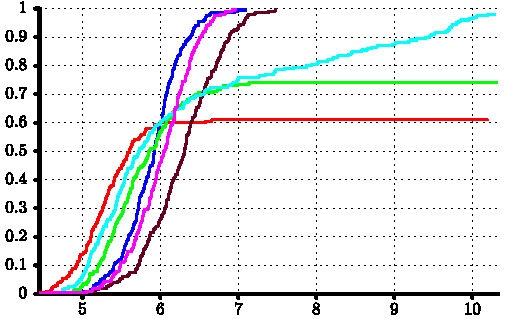
\includegraphics[width=0.234375\paperwidth]{graphics/maxsat_example/ECDF_log_10_RT_F_k_0_01_distinct_n/SigAlternate_ECDF_log_10_RT_F_k_0_01_distinct_n_20}%
\\\scriptsize{$\maxSatVariables=20$}}%
}{0.50625}{0.18}%
%
\locate{3-}{%
\parbox{0.234375\paperwidth}{\centering%
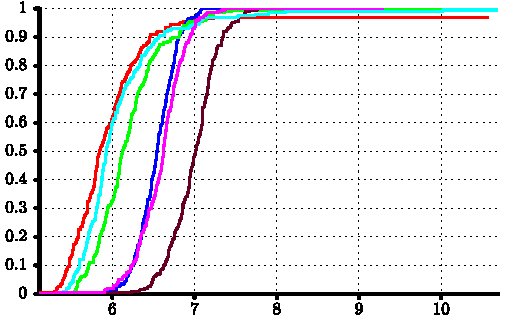
\includegraphics[width=0.234375\paperwidth]{graphics/maxsat_example/ECDF_log_10_RT_F_k_0_01_distinct_n/SigAlternate_ECDF_log_10_RT_F_k_0_01_distinct_n_50}%
\\\scriptsize{$\maxSatVariables=50$}}%
}{0.753125}{0.18}%
%
\locate{4-}{%
\parbox{0.234375\paperwidth}{\centering%
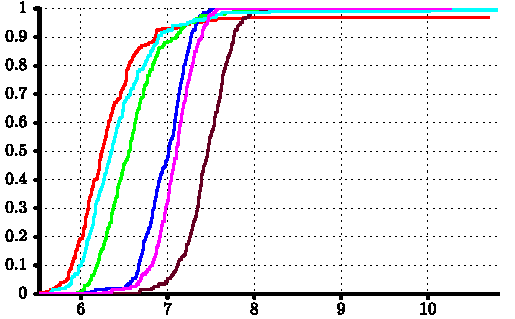
\includegraphics[width=0.234375\paperwidth]{graphics/maxsat_example/ECDF_log_10_RT_F_k_0_01_distinct_n/SigAlternate_ECDF_log_10_RT_F_k_0_01_distinct_n_75}%
\\\scriptsize{$\maxSatVariables=75$}}%
}{0.0125}{0.443333333333333}%
%
\locate{5-}{%
\parbox{0.234375\paperwidth}{\centering%
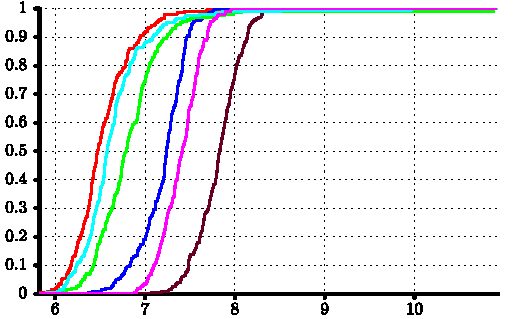
\includegraphics[width=0.234375\paperwidth]{graphics/maxsat_example/ECDF_log_10_RT_F_k_0_01_distinct_n/SigAlternate_ECDF_log_10_RT_F_k_0_01_distinct_n_100}%
\\\scriptsize{$\maxSatVariables=100$}}%
}{0.259375}{0.443333333333333}%
%
\locate{6-}{%
\parbox{0.234375\paperwidth}{\centering%
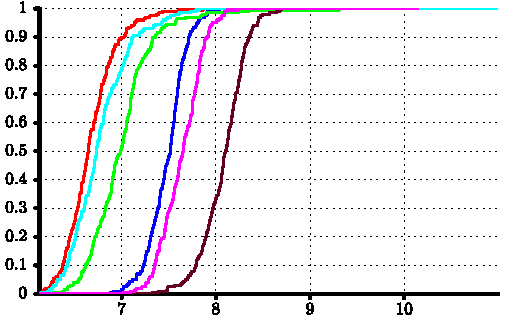
\includegraphics[width=0.234375\paperwidth]{graphics/maxsat_example/ECDF_log_10_RT_F_k_0_01_distinct_n/SigAlternate_ECDF_log_10_RT_F_k_0_01_distinct_n_125}%
\\\scriptsize{$\maxSatVariables=125$}}%
}{0.50625}{0.443333333333333}%
%
\locate{7-}{%
\parbox{0.234375\paperwidth}{\centering%
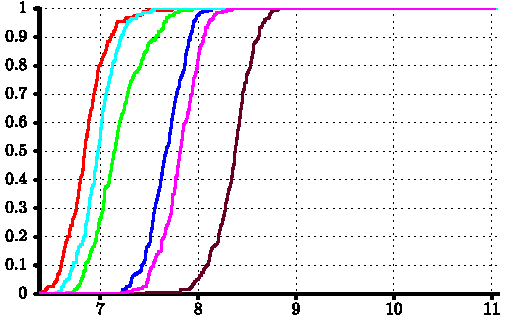
\includegraphics[width=0.234375\paperwidth]{graphics/maxsat_example/ECDF_log_10_RT_F_k_0_01_distinct_n/SigAlternate_ECDF_log_10_RT_F_k_0_01_distinct_n_150}%
\\\scriptsize{$\maxSatVariables=150$}}%
}{0.753125}{0.443333333333333}%
%
\locate{8-}{%
\parbox{0.234375\paperwidth}{\centering%
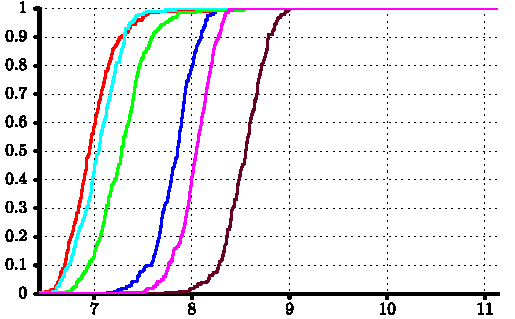
\includegraphics[width=0.234375\paperwidth]{graphics/maxsat_example/ECDF_log_10_RT_F_k_0_01_distinct_n/SigAlternate_ECDF_log_10_RT_F_k_0_01_distinct_n_175}%
\\\scriptsize{$\maxSatVariables=175$}}%
}{0.0125}{0.706666666666667}%
%
\locate{9-}{%
\parbox{0.234375\paperwidth}{\centering%
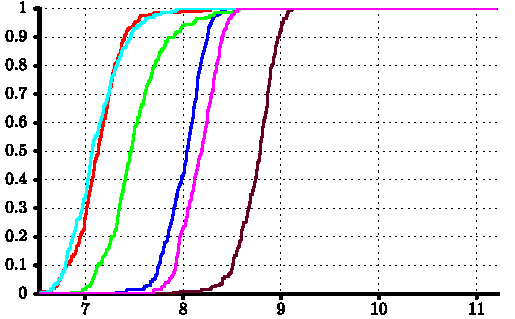
\includegraphics[width=0.234375\paperwidth]{graphics/maxsat_example/ECDF_log_10_RT_F_k_0_01_distinct_n/SigAlternate_ECDF_log_10_RT_F_k_0_01_distinct_n_200}%
\\\scriptsize{$\maxSatVariables=200$}}%
}{0.259375}{0.706666666666667}%%
%
\locate{10-}{%
\parbox{0.234375\paperwidth}{\centering%
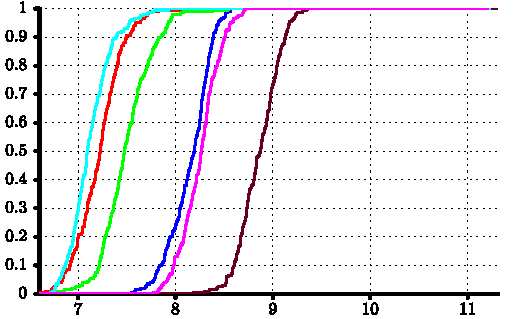
\includegraphics[width=0.234375\paperwidth]{graphics/maxsat_example/ECDF_log_10_RT_F_k_0_01_distinct_n/SigAlternate_ECDF_log_10_RT_F_k_0_01_distinct_n_225}%
\\\scriptsize{$\maxSatVariables=225$}}%
}{0.50625}{0.706666666666667}%
%
\locate{11-}{%
\parbox{0.234375\paperwidth}{\centering%
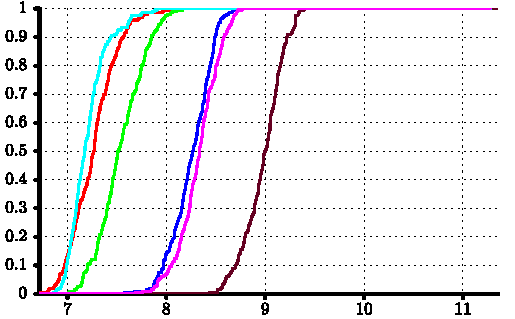
\includegraphics[width=0.234375\paperwidth]{graphics/maxsat_example/ECDF_log_10_RT_F_k_0_01_distinct_n/SigAlternate_ECDF_log_10_RT_F_k_0_01_distinct_n_250}%
\\\scriptsize{$\maxSatVariables=250$}}%
}{0.753125}{0.706666666666667}%
%
\end{frame}%
%
%
\begin{frame}%
\frametitle{Progress for Different Values of \scalebox{1.3}{\ensuremath{\mathbf{\maxSatClauses}}}}%
%
\locate{1-}{%
\parbox{0.234\paperwidth}{\raggedright\small{%
\only<-1>{We now look at the progress curves (\measureObjectiveValue\ over \measureFEs\ divided by\footnote<1>{We normalize \measureFEs\ with \maxSatVariables\ in the hope to make the time measure comparable over different \maxSatVariables.} \maxSatVariables, log-scaled) for different values of \maxSatClauses.}%
\only<2>{For very small-scale problems, all algorithms behave similar.}%
\only<3>{But soon, two groups form: with and without restarts.}%
\only<4>{Algorithms using \emph{my example restart policy} seem to be slower.}%
\only<5>{The gap increases with rising \maxSatClauses}%
\only<6>{Thus, we find: algorithms with my restart policy are slower than those without\dots}%
\only<7>{{\dots}but from the ECDF we know they can solve more problems eventually.}%
\only<8>{For all scales, the initial random solutions, seem to have about 12\% of unsatisfied clauses (in median).}%
\only<9->{Convergence seems to happen between 100\maxSatVariables\ and 1000\maxSatVariables}%
}}}{0.013}{0.187}%
%
\locate{1-}{%
\parbox{0.234375\paperwidth}{\centering%
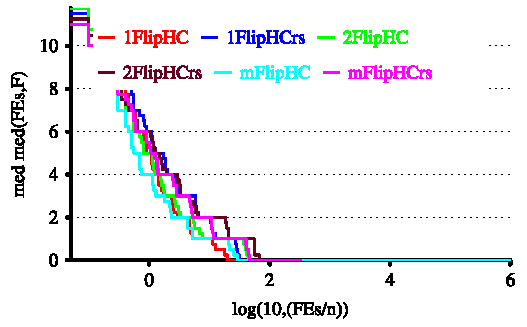
\includegraphics[width=0.234375\paperwidth]{graphics/maxsat_example/med_med_log_10_FEs_n_F_distinct_k/IEEEtran_med_med_log_10_FEs_n_F_distinct_k_legend}%
\\\scriptsize{legend}}%
}{0.259375}{0.18}%
%
\locate{2-}{%
\parbox{0.234375\paperwidth}{\centering%
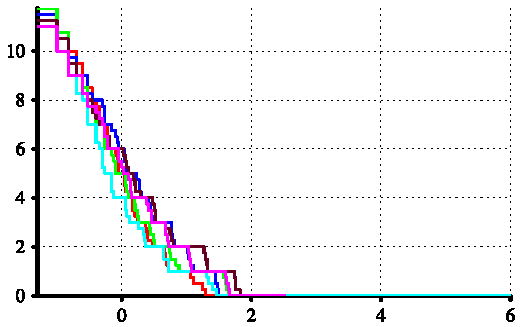
\includegraphics[width=0.234375\paperwidth]{graphics/maxsat_example/med_med_log_10_FEs_n_F_distinct_k/IEEEtran_med_med_log_10_FEs_n_F_distinct_k_91}%
\\\scriptsize{$\maxSatClauses=91$}}%
}{0.50625}{0.18}%
%
\locate{3-}{%
\parbox{0.234375\paperwidth}{\centering%
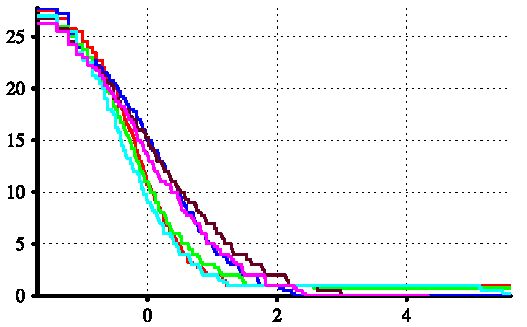
\includegraphics[width=0.234375\paperwidth]{graphics/maxsat_example/med_med_log_10_FEs_n_F_distinct_k/IEEEtran_med_med_log_10_FEs_n_F_distinct_k_218}%
\\\scriptsize{$\maxSatClauses=218$}}%
}{0.753125}{0.18}%
%
\locate{4-}{%
\parbox{0.234375\paperwidth}{\centering%
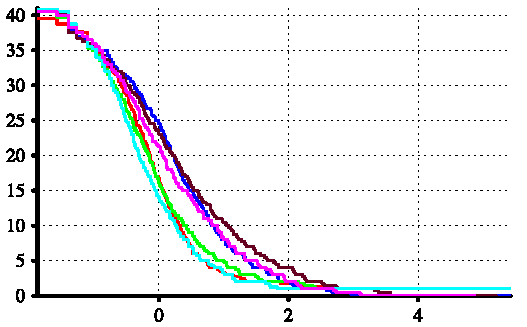
\includegraphics[width=0.234375\paperwidth]{graphics/maxsat_example/med_med_log_10_FEs_n_F_distinct_k/IEEEtran_med_med_log_10_FEs_n_F_distinct_k_325}%
\\\scriptsize{$\maxSatClauses=325$}}%
}{0.0125}{0.443333333333333}%
%
\locate{5-}{%
\parbox{0.234375\paperwidth}{\centering%
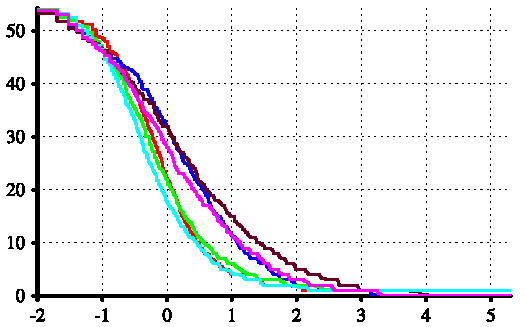
\includegraphics[width=0.234375\paperwidth]{graphics/maxsat_example/med_med_log_10_FEs_n_F_distinct_k/IEEEtran_med_med_log_10_FEs_n_F_distinct_k_430}%
\\\scriptsize{$\maxSatClauses=430$}}%
}{0.259375}{0.443333333333333}%
%
\locate{6-}{%
\parbox{0.234375\paperwidth}{\centering%
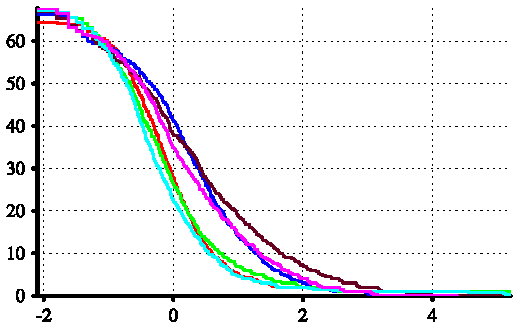
\includegraphics[width=0.234375\paperwidth]{graphics/maxsat_example/med_med_log_10_FEs_n_F_distinct_k/IEEEtran_med_med_log_10_FEs_n_F_distinct_k_538}%
\\\scriptsize{$\maxSatClauses=538$}}%
}{0.50625}{0.443333333333333}%
%
\locate{7-}{%
\parbox{0.234375\paperwidth}{\centering%
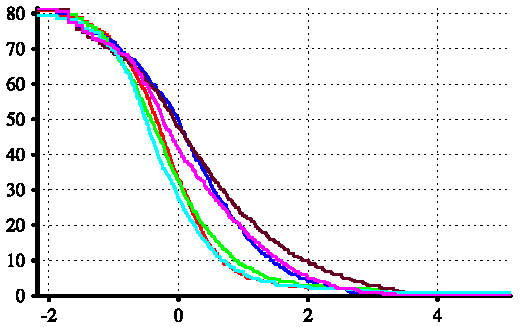
\includegraphics[width=0.234375\paperwidth]{graphics/maxsat_example/med_med_log_10_FEs_n_F_distinct_k/IEEEtran_med_med_log_10_FEs_n_F_distinct_k_645}%
\\\scriptsize{$\maxSatClauses=645$}}%
}{0.753125}{0.443333333333333}%
%
\locate{8-}{%
\parbox{0.234375\paperwidth}{\centering%
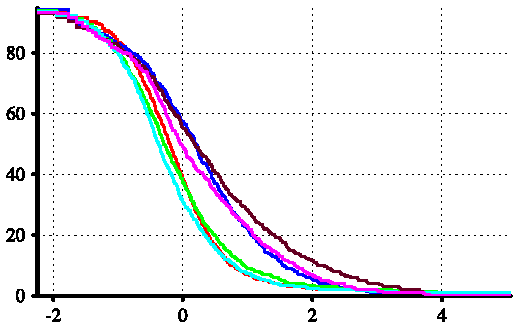
\includegraphics[width=0.234375\paperwidth]{graphics/maxsat_example/med_med_log_10_FEs_n_F_distinct_k/IEEEtran_med_med_log_10_FEs_n_F_distinct_k_753}%
\\\scriptsize{$\maxSatClauses=753$}}%
}{0.0125}{0.706666666666667}%
%
\locate{9-}{%
\parbox{0.234375\paperwidth}{\centering%
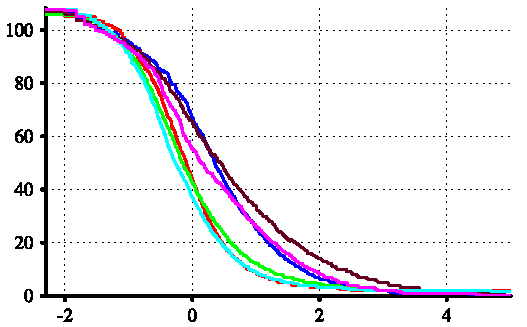
\includegraphics[width=0.234375\paperwidth]{graphics/maxsat_example/med_med_log_10_FEs_n_F_distinct_k/IEEEtran_med_med_log_10_FEs_n_F_distinct_k_860}%
\\\scriptsize{$\maxSatClauses=860$}}%
}{0.259375}{0.706666666666667}%%
%
\locate{10-}{%
\parbox{0.234375\paperwidth}{\centering%
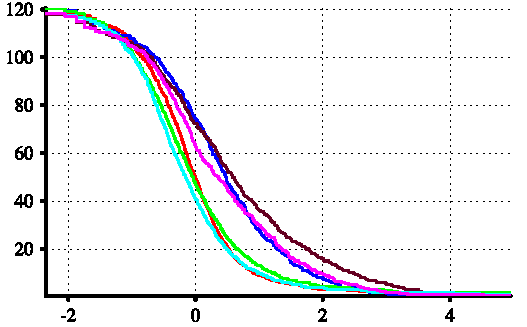
\includegraphics[width=0.234375\paperwidth]{graphics/maxsat_example/med_med_log_10_FEs_n_F_distinct_k/IEEEtran_med_med_log_10_FEs_n_F_distinct_k_960}%
\\\scriptsize{$\maxSatClauses=960$}}%
}{0.50625}{0.706666666666667}%
%
\locate{11-}{%
\parbox{0.234375\paperwidth}{\centering%
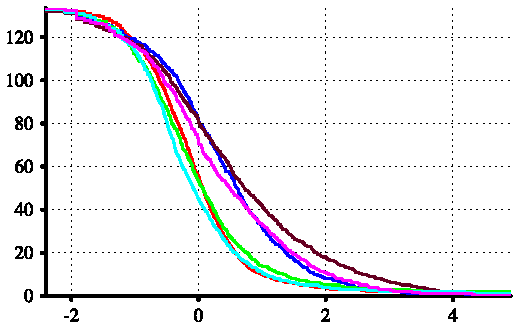
\includegraphics[width=0.234375\paperwidth]{graphics/maxsat_example/med_med_log_10_FEs_n_F_distinct_k/IEEEtran_med_med_log_10_FEs_n_F_distinct_k_1065}%
\\\scriptsize{$\maxSatClauses=1065$}}%
}{0.753125}{0.706666666666667}%
%
\end{frame}%
%
%
\begin{frame}%
\frametitle{StdDev of \measureObjectiveValue\ for Different Values of \scalebox{1.3}{\ensuremath{\mathbf{\maxSatVariables}}}}%
%
\locate{1-}{%
\parbox{0.234\paperwidth}{\raggedright\small{%
\only<-1>{Let's look at the standard deviation of the best objective value \measureObjectiveValue\ (divided by\footnote<1>{Since \measureObjectiveValue\ is always in $1\dots\maxSatClauses$, dividing it by \maxSatClauses\ normalizes it into $[0,1]$ and makes the values comparable for different \maxSatClauses\ or \maxSatVariables.} \maxSatClauses) found over \measureRuntime\ (log-scaled) for different values of \maxSatVariables.}%
\only<2>{For small-scale problems, the standard deviation seems to decrease steadily.}%
\only<3>{The reason is probably that the algorithms converge nicely.}%
\only<4>{For the methods with restarts, it reaches very close to 0.}%
\only<5>{For those without, it remains constant above 0 after some time.}%
\only<6>{These algorithms probably get stuck at different local optima in different runs.}%
\only<7>{For increasing scales, the standard deviation goes first down, then up, then farther down.}%
\only<8>{Maybe there is some kind of hard-to-attain improvement that some runs find earlier than others.}%
\only<9>{The time of convergence seems to increase for the methods with restarts with \maxSatVariables.}%
\only<10->{The early standard deviations are usually below 0.03 and highest for small \maxSatVariables.}% 
}}}{0.013}{0.187}%
%
\locate{1-}{%
\parbox{0.234375\paperwidth}{\centering%
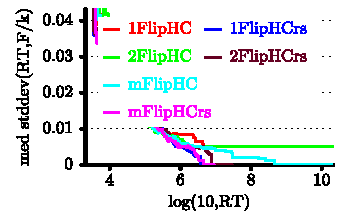
\includegraphics[width=0.234375\paperwidth]{graphics/maxsat_example/med_stddev_log_10_RT_F_k_distinct_n/LNCS_med_stddev_log_10_RT_F_k_distinct_n_legend}%
\\\scriptsize{legend}}%
}{0.259375}{0.18}%
%
\locate{2-}{%
\parbox{0.234375\paperwidth}{\centering%
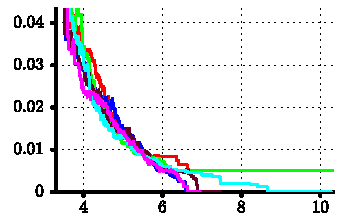
\includegraphics[width=0.234375\paperwidth]{graphics/maxsat_example/med_stddev_log_10_RT_F_k_distinct_n/LNCS_med_stddev_log_10_RT_F_k_distinct_n_20}%
\\\scriptsize{$\maxSatVariables=20$}}%
}{0.50625}{0.18}%
%
\locate{3-}{%
\parbox{0.234375\paperwidth}{\centering%
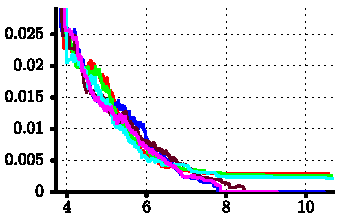
\includegraphics[width=0.234375\paperwidth]{graphics/maxsat_example/med_stddev_log_10_RT_F_k_distinct_n/LNCS_med_stddev_log_10_RT_F_k_distinct_n_50}%
\\\scriptsize{$\maxSatVariables=50$}}%
}{0.753125}{0.18}%
%
\locate{4-}{%
\parbox{0.234375\paperwidth}{\centering%
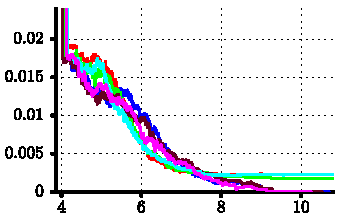
\includegraphics[width=0.234375\paperwidth]{graphics/maxsat_example/med_stddev_log_10_RT_F_k_distinct_n/LNCS_med_stddev_log_10_RT_F_k_distinct_n_75}%
\\\scriptsize{$\maxSatVariables=75$}}%
}{0.0125}{0.443333333333333}%
%
\locate{5-}{%
\parbox{0.234375\paperwidth}{\centering%
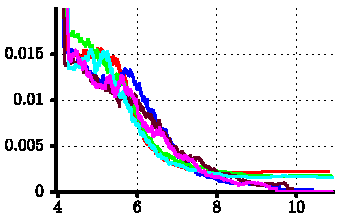
\includegraphics[width=0.234375\paperwidth]{graphics/maxsat_example/med_stddev_log_10_RT_F_k_distinct_n/LNCS_med_stddev_log_10_RT_F_k_distinct_n_100}%
\\\scriptsize{$\maxSatVariables=100$}}%
}{0.259375}{0.443333333333333}%
%
\locate{6-}{%
\parbox{0.234375\paperwidth}{\centering%
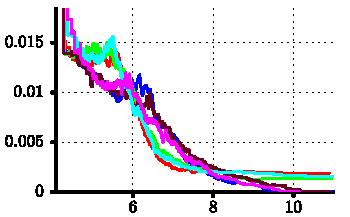
\includegraphics[width=0.234375\paperwidth]{graphics/maxsat_example/med_stddev_log_10_RT_F_k_distinct_n/LNCS_med_stddev_log_10_RT_F_k_distinct_n_125}%
\\\scriptsize{$\maxSatVariables=125$}}%
}{0.50625}{0.443333333333333}%
%
\locate{7-}{%
\parbox{0.234375\paperwidth}{\centering%
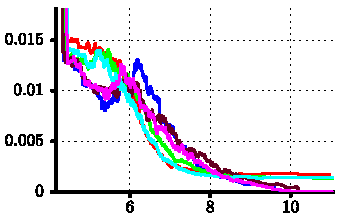
\includegraphics[width=0.234375\paperwidth]{graphics/maxsat_example/med_stddev_log_10_RT_F_k_distinct_n/LNCS_med_stddev_log_10_RT_F_k_distinct_n_150}%
\\\scriptsize{$\maxSatVariables=150$}}%
}{0.753125}{0.443333333333333}%
%
\locate{8-}{%
\parbox{0.234375\paperwidth}{\centering%
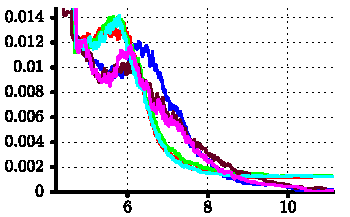
\includegraphics[width=0.234375\paperwidth]{graphics/maxsat_example/med_stddev_log_10_RT_F_k_distinct_n/LNCS_med_stddev_log_10_RT_F_k_distinct_n_175}%
\\\scriptsize{$\maxSatVariables=175$}}%
}{0.0125}{0.706666666666667}%
%
\locate{9-}{%
\parbox{0.234375\paperwidth}{\centering%
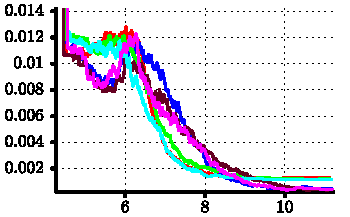
\includegraphics[width=0.234375\paperwidth]{graphics/maxsat_example/med_stddev_log_10_RT_F_k_distinct_n/LNCS_med_stddev_log_10_RT_F_k_distinct_n_200}%
\\\scriptsize{$\maxSatVariables=200$}}%
}{0.259375}{0.706666666666667}%%
%
\locate{10-}{%
\parbox{0.234375\paperwidth}{\centering%
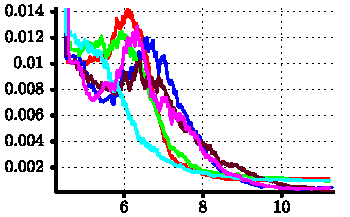
\includegraphics[width=0.234375\paperwidth]{graphics/maxsat_example/med_stddev_log_10_RT_F_k_distinct_n/LNCS_med_stddev_log_10_RT_F_k_distinct_n_225}%
\\\scriptsize{$\maxSatVariables=225$}}%
}{0.50625}{0.706666666666667}%
%
\locate{11-}{%
\parbox{0.234375\paperwidth}{\centering%
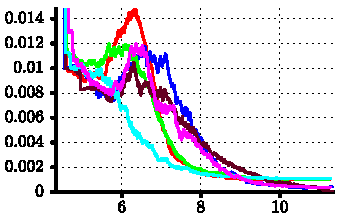
\includegraphics[width=0.234375\paperwidth]{graphics/maxsat_example/med_stddev_log_10_RT_F_k_distinct_n/LNCS_med_stddev_log_10_RT_F_k_distinct_n_250}%
\\\scriptsize{$\maxSatVariables=250$}}%
}{0.753125}{0.706666666666667}%
%
\end{frame}%
%
%%
%
\begin{frame}[t]%
\frametitle{Result}%
\only<-5>{%
\begin{itemize}%
\item The Evaluator will now produce report documents containing the requested information (and figures)%
\end{itemize}%
}%
\locate{6}{%
\parbox{\paperwidth}{%
\centering\scalebox{1.8}{\hyperlink{maxSatInteractiveDemoEnd}{\beamergotobutton{continue after end of interactive demo slides}}}%
}%
}{0}{0.16}%
%
\locateWithCaption{2-}{%
\strut\vbox to 0.475\paperheight{\vfil\fbox{%
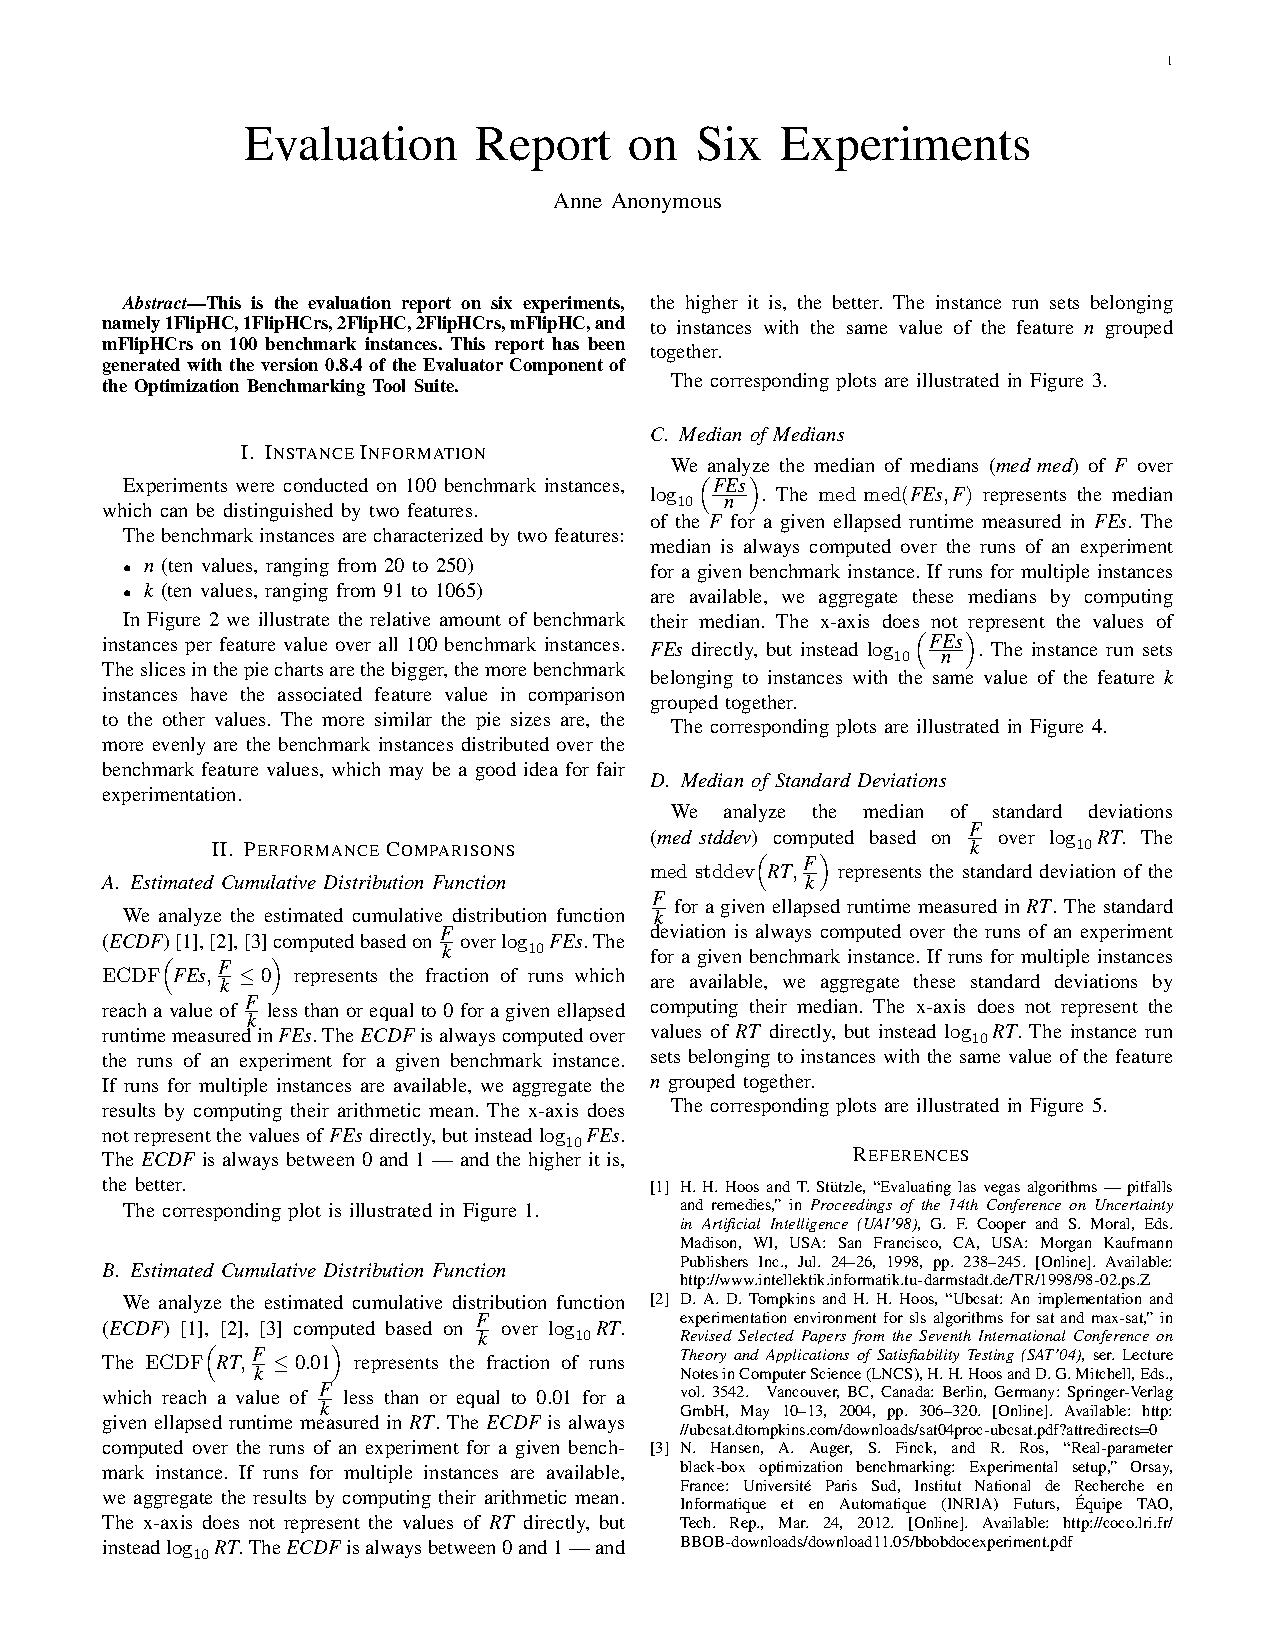
\includegraphics[width=0.215\paperwidth,page=1]{graphics/maxsat_example/maxsat_example_reports/IEEEtran_report.pdf}%
}\strut\hfill\strut}%
}{%
first page of the report in \LaTeX\ for \texttt{IEEEtran}%
}{0.02}{0.255}{0.225}%
%
%
\locateWithCaption{3-}{%
\strut\vbox to 0.475\paperheight{\vfil\fbox{%
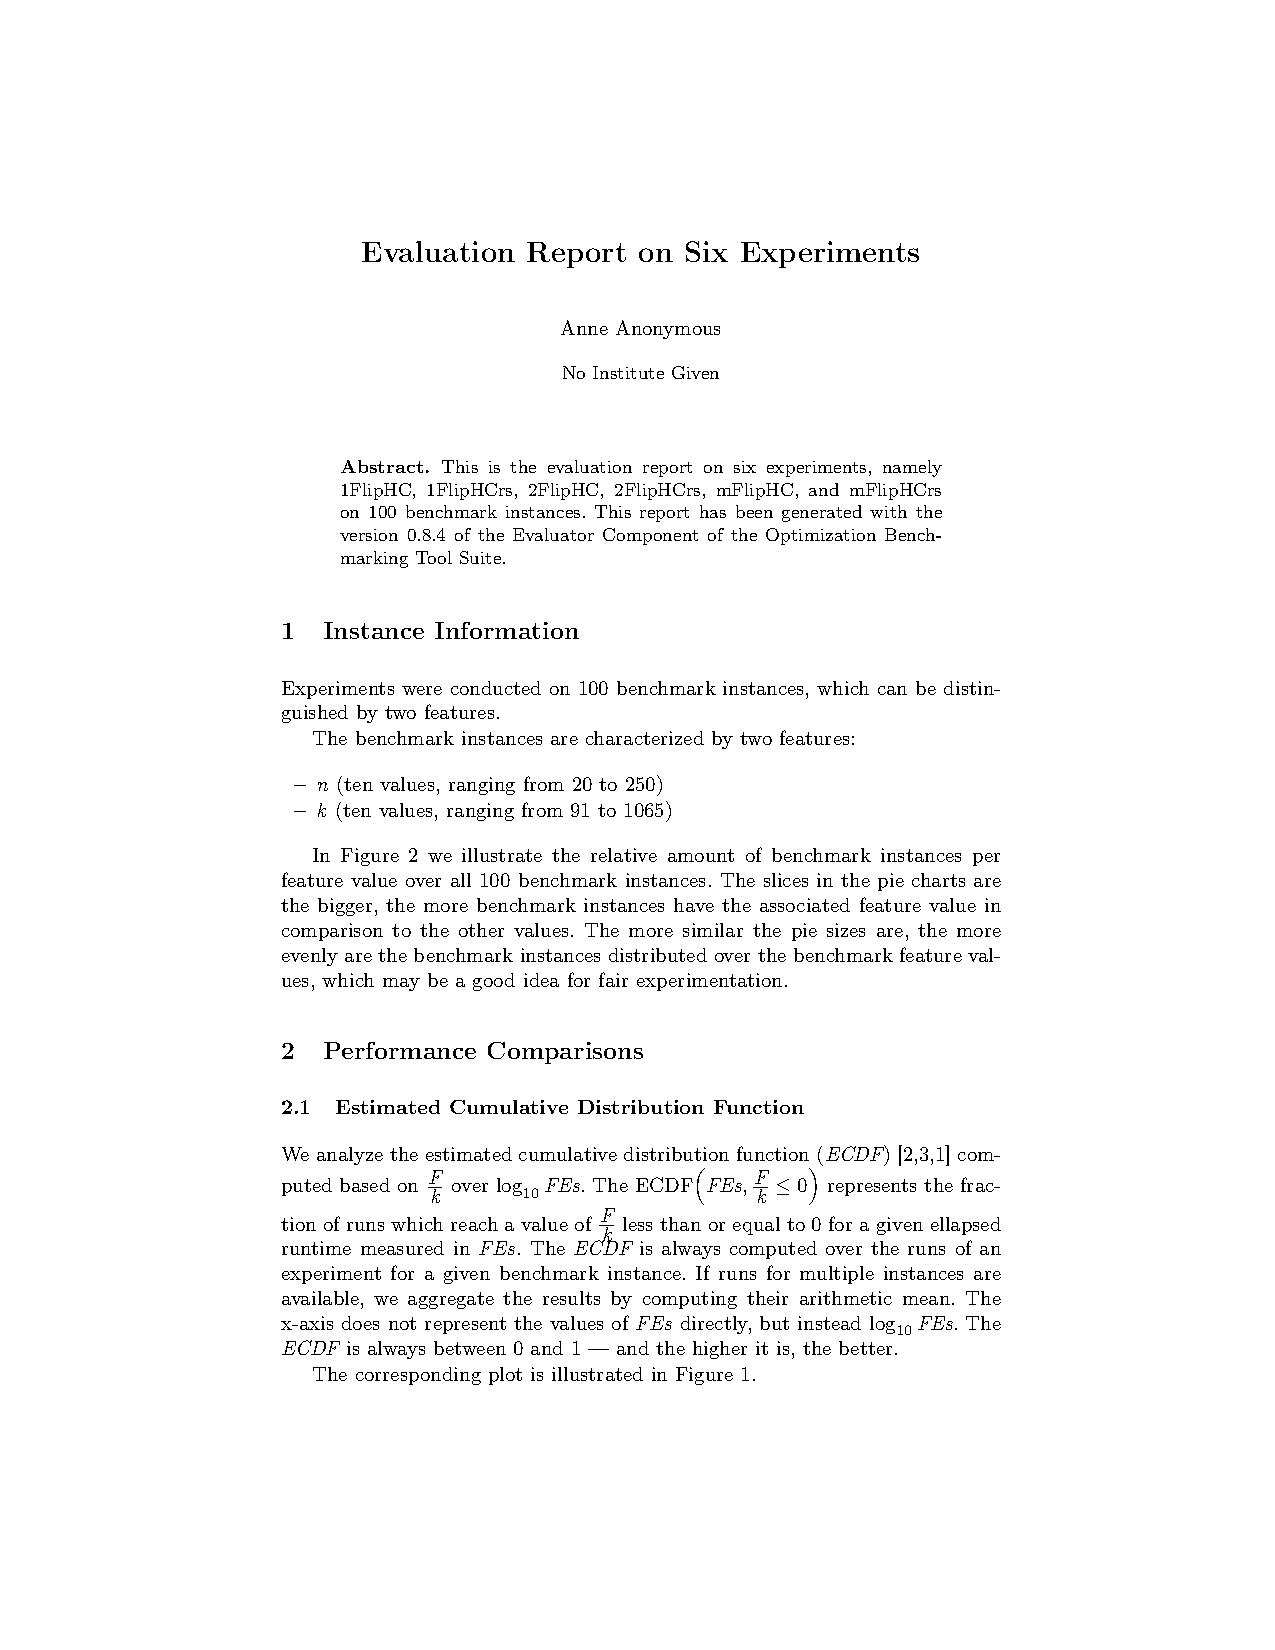
\includegraphics[width=0.215\paperwidth,page=1]{graphics/maxsat_example/maxsat_example_reports/LNCS_report.pdf}%
}\strut\hfill\strut}%
}{%
first page of the report in \LaTeX\ for \texttt{LNCS}%
}{0.265}{0.255}{0.225}%
%
\locateWithCaption{4-}{%
\strut\vbox to 0.475\paperheight{\vfil\fbox{%
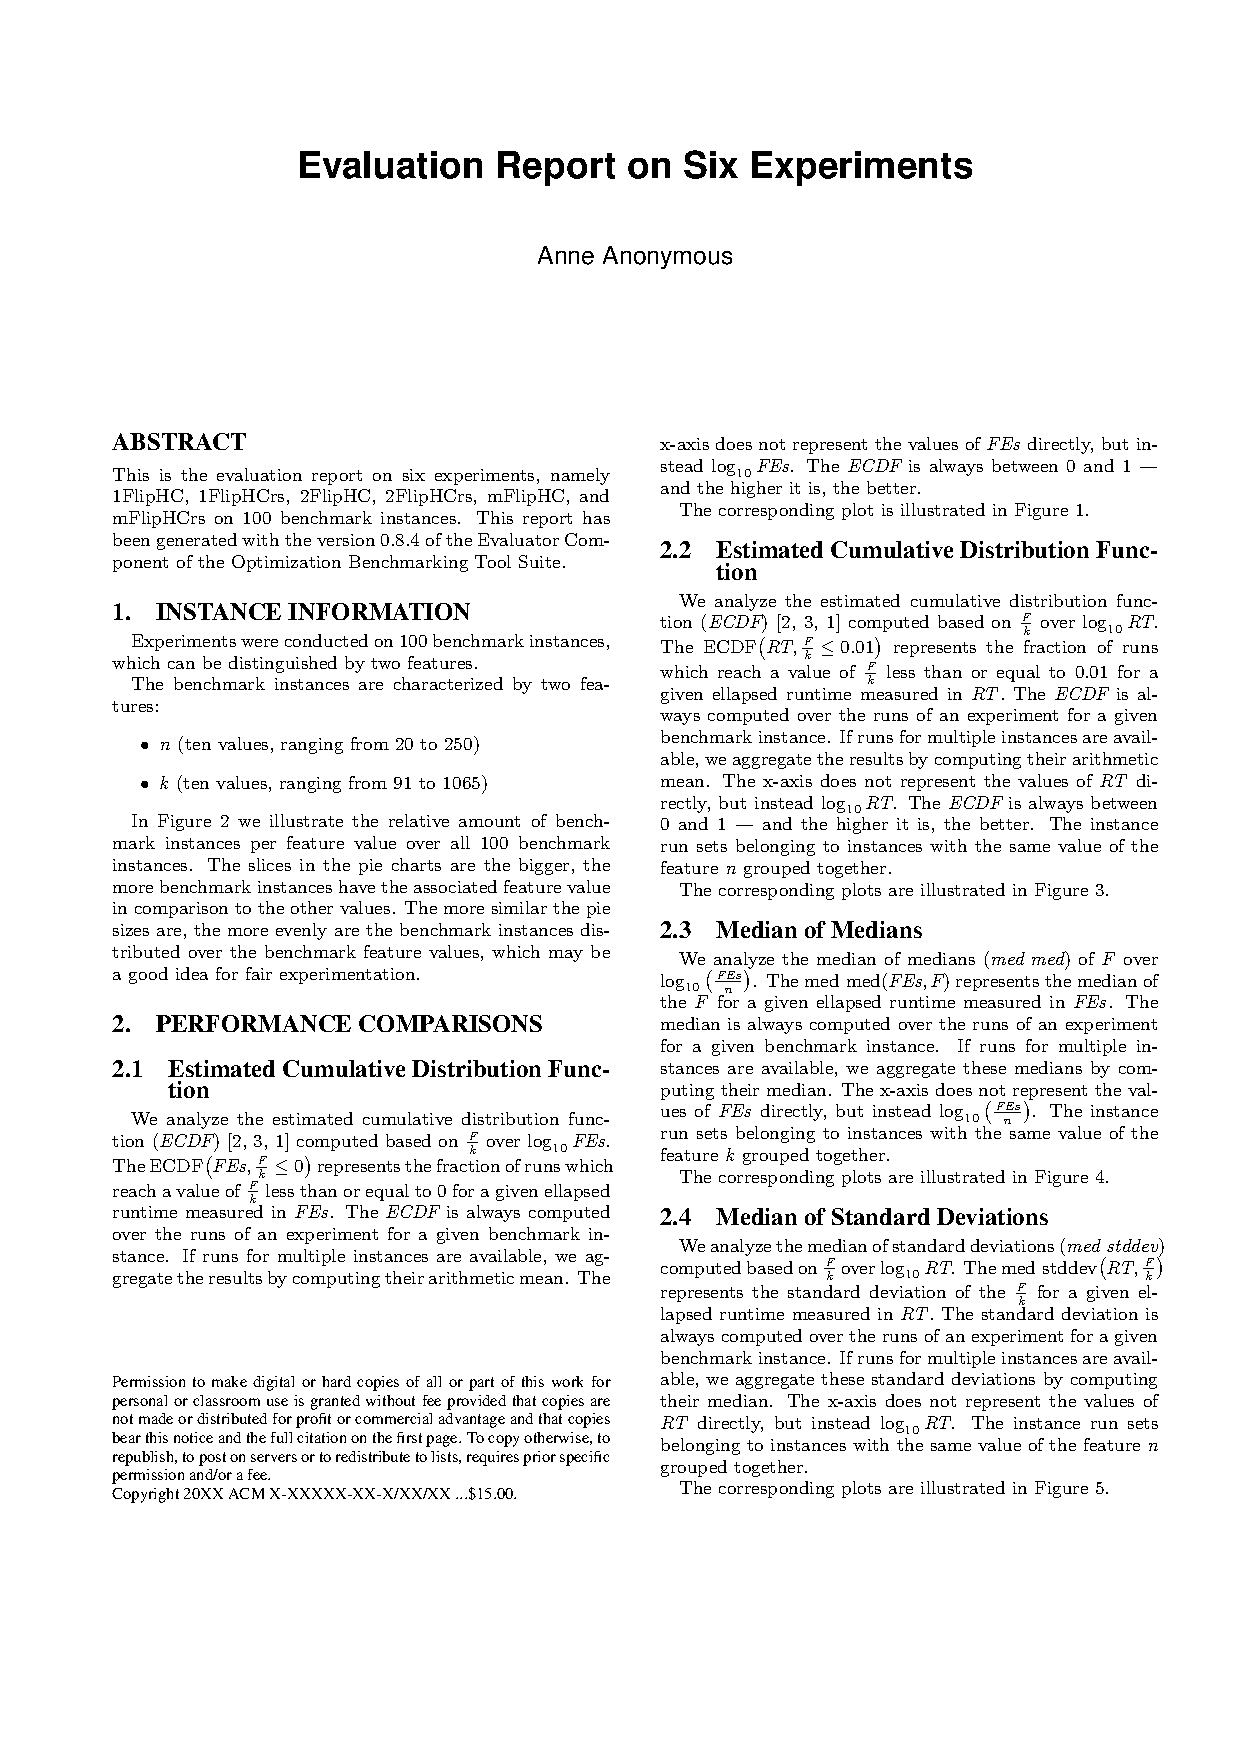
\includegraphics[width=0.215\paperwidth,page=1]{graphics/maxsat_example/maxsat_example_reports/SigAlternate_report.pdf}%
}\strut\hfill\strut}%
}{%
first page of the report in \LaTeX\ for \texttt{sig-alternate}%
}{0.51}{0.255}{0.225}%
%
\locateWithCaption{5-}{%
\strut\vbox to 0.475\paperheight{\vfil\fbox{%
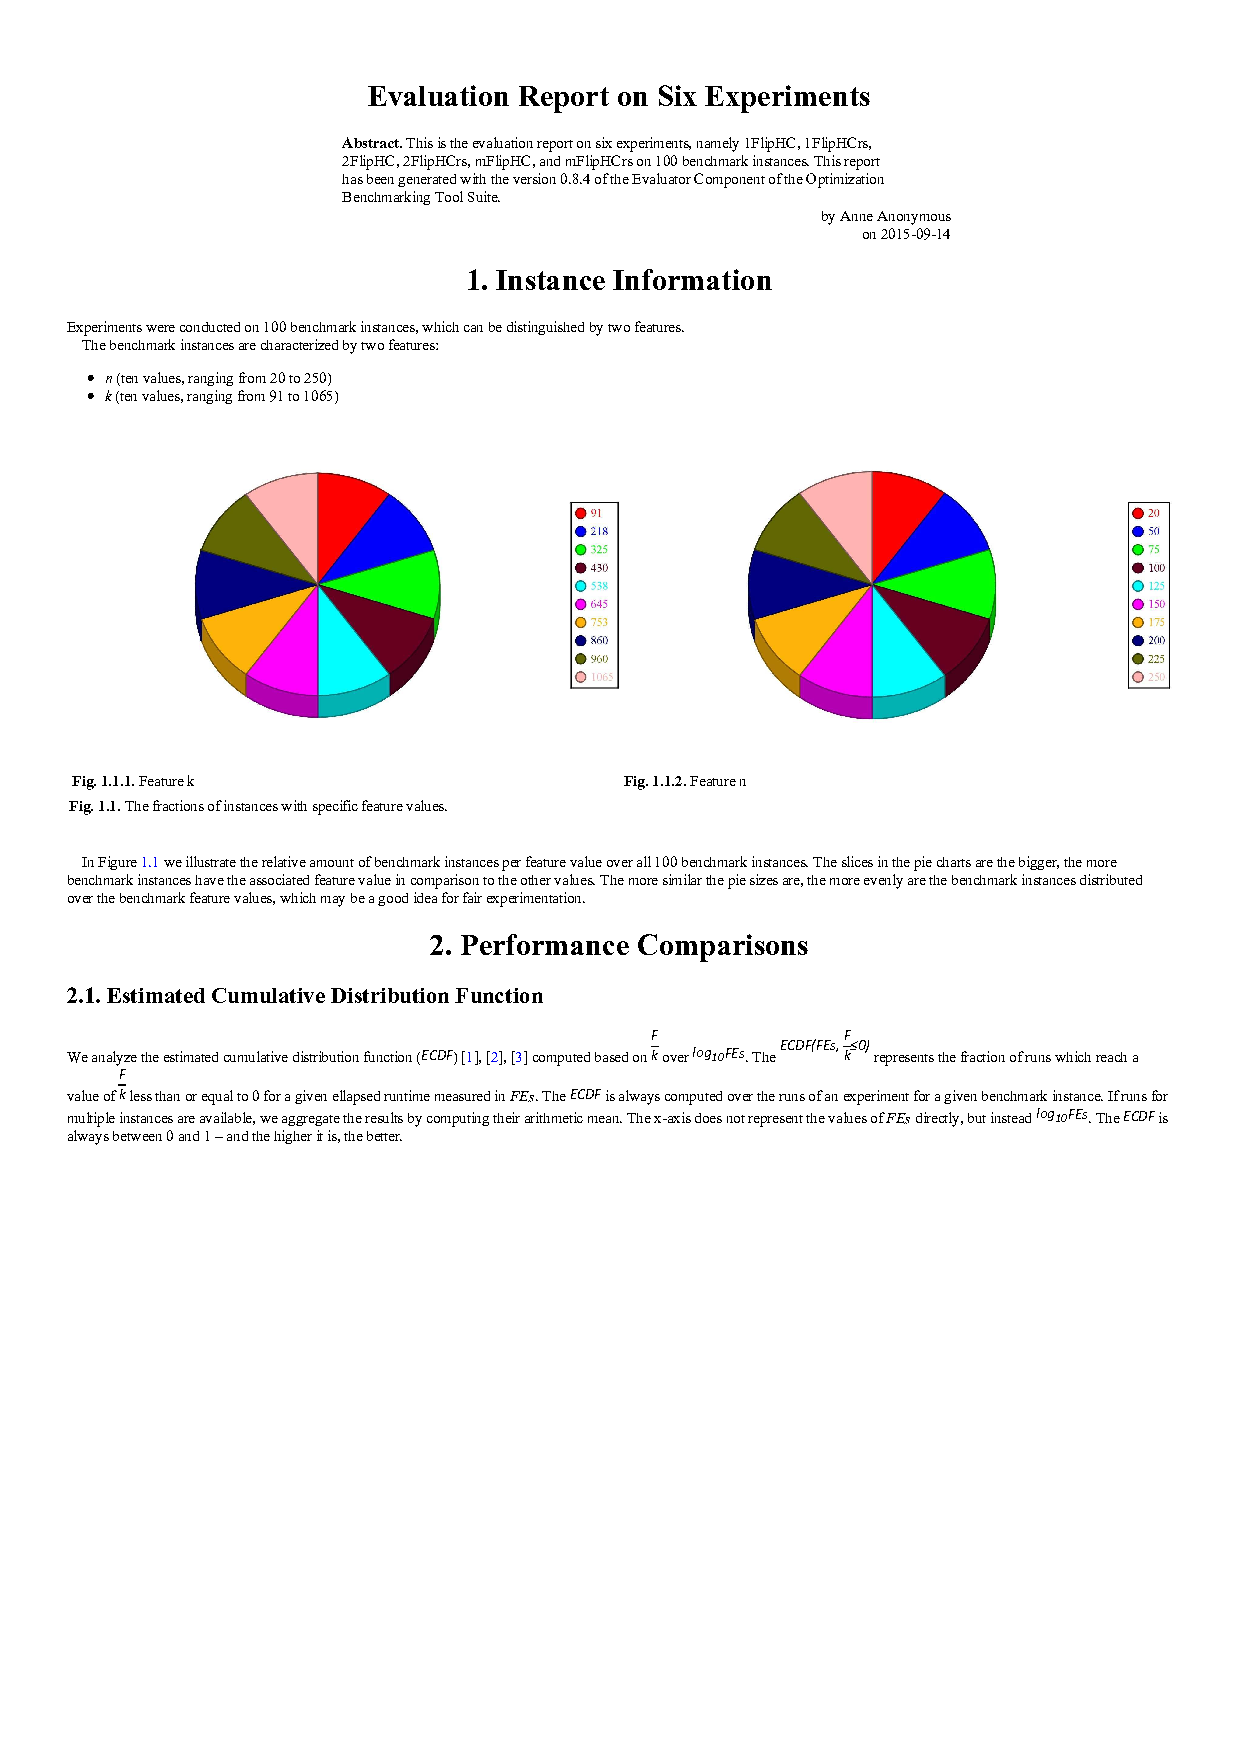
\includegraphics[width=0.215\paperwidth,page=1]{graphics/maxsat_example/maxsat_example_reports/XHTML_report.pdf}%
}\strut\hfill\strut}%
}{%
first page of the report in \texttt{XHTML}%
}{0.755}{0.255}{0.225}%
%
\end{frame}%
%
%